%!TEX TS-program = xelatex
\documentclass[]{friggeri-cv}
% if you want to add fontawesome package
% you need to compile the tex file with LuaLaTeX
% References:
%   http://texdoc.net/texmf-dist/doc/latex/fontawesome/fontawesome.pdf
%   https://www.ctan.org/tex-archive/fonts/fontawesome?lang=en
\hypersetup{
    pdftitle={},
    pdfauthor={},
    pdfsubject={},
    pdfkeywords={},
    colorlinks,
    allbordercolors=white       % white border color for all
}

\newcommand{\changeurlcolor}[1]{\hypersetup{urlcolor=#1}}       
\smartdiagramset{
    bubble center node font = \footnotesize,
    bubble node font = \footnotesize,
    % specifies the minimum size of the bubble center node
    bubble center node size = 0.5cm,
    %  specifies the minimum size of the bubbles
    bubble node size = 0.5cm,
    % specifies which is the distance among the bubble center node and the other bubbles
    distance center/other bubbles = 0.3cm,
    % sets the distance from the text to the border of the bubble center node
    distance text center bubble = 0.5cm,
    % set center bubble color
    bubble center node color = pblue,
    % define the list of colors usable in the diagram
    set color list = {lightgray, materialcyan, orange, green, materialorange, materialteal, materialamber, materialindigo, materialgreen, materiallime},
    % sets the opacity at which the bubbles are shown
    bubble fill opacity = 0.6,
    % sets the opacity at which the bubble text is shown
    bubble text opacity = 0.5,
}

\addbibresource{bibliography.bib}

% Programming skill bars

\programming{{SQL $\textbullet$ MDX / 3}, {BASH / 3},{C $\textbullet$ C++ / 2}, {JavaScript / 3},{Java / 4.5}}


\begin{document}
\makeprofile %Print the side bar

\header{Mahieddine}{Dellabani}{Technical Lead}
      
% Fake text to add separator      
\fcolorbox{white}{gray}{\parbox{\dimexpr\textwidth-2\fboxsep-2\fboxrule}{%
.....
}}

% In the aside, each new line forces a line break
%\begin{aside2}
%  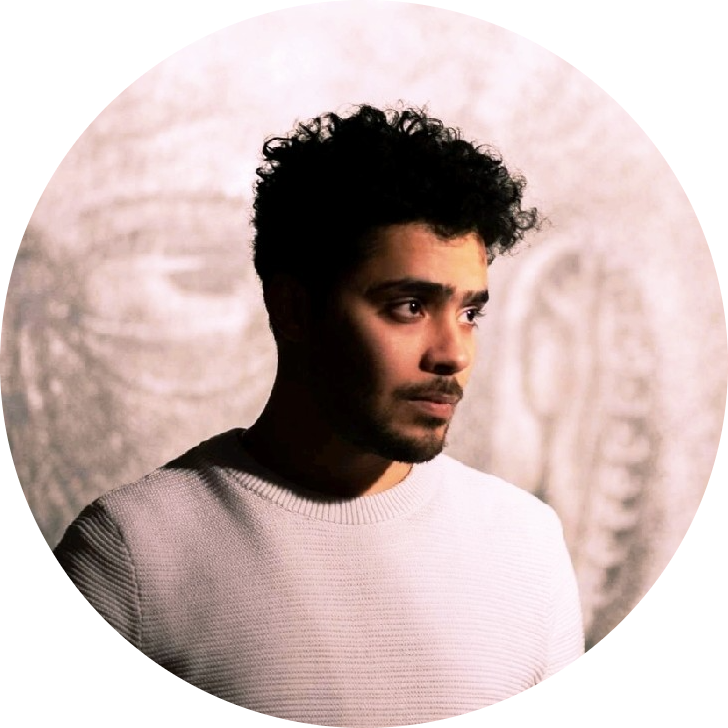
\includegraphics[scale=0.35]{img/mdellabani}
%  \section{Address}
%     Castel Black
%     Winterfell, Far North
%     ~
%   \section{Tel \& Skype}
%     +00 000 000000
%     johnsnow.skype
%     ~
%   \section{Mail}
%     \href{mailto:john.snow@castelblack.com}{\textbf{john.snow@}\\castelblack.com}
%     ~
%   \section{Web \& Git}
%     \href{http://mywebsite.com}{mywebsite.com}
%     \href{https://bitbucket.org/mygit}{bitbucket.org/mygit}
%     \href{https://github.com/mygit}{github.com/mygit}
%     \href{https://gitlab.com/u/mygit}{gitlab.com/u/mygit}
%     ~
  % use  \hspace{} or \vspace{} to change bubble size, if needed
%   \section{Programming}
%     \smartdiagram[bubble diagram]{
%         \textbf{C/C++},
%         \textbf{Python},
%         \textbf{Java},
%         \textbf{Lua/UCI},
%         \textbf{Other\vspace{3mm}},
%         \textbf{HTML/CSS}\\\textbf{JS/jQuery},
%         \textbf{PHP},
%         \textbf{Android},
%         \textbf{Bash}
%     }
%     ~
%   \section{Personal Skills}
%     \smartdiagram[bubble diagram]{
%         \textbf{Team}\\\textbf{Player},
%         \textbf{Initiative},
%         \textbf{Curiosity},
%         \textbf{Problem}\\\textbf{Solving},
%         \textbf{\vspace{2mm}Manage\vspace{2mm}},
%         \textbf{Organize}
%     }
%     ~
% \end{aside2}
% ~
\begin{textblock}{6}(0.5, 0.2)
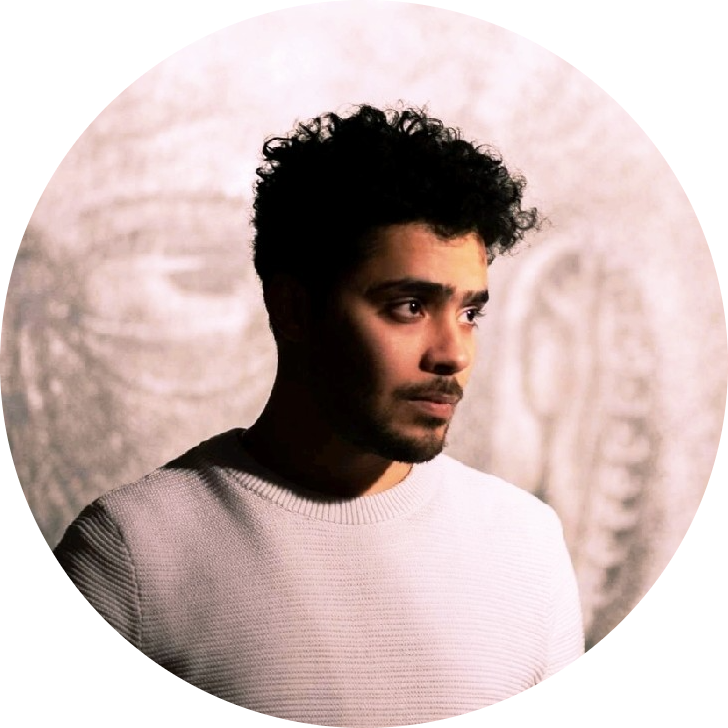
\includegraphics[scale=0.18]{img/mdellabani}


%\profile
  \begin{tabular}{c p{5cm}}
    \raisebox{-6pt}{\Large{\textifsymbol{18} $\quad$}} &  \small{ 994 route de Damoulens} \\ % Address
    \vspace*{2mm}
    \raisebox{-4pt}{} & \small{40320, Bahus-Soubiran} \\ % Address
    \raisebox{-1pt}{\hspace{-1mm}\Large{\faMobile}$\quad$} & \small{+33 6 05 83 31 66} \\ % Phone number
    \vspace*{0.5mm}
  \end{tabular}
  \newline
  \hspace*{10mm}\href{mailto:mahieddine.dellabani@gmail.com}{\Large{\textcolor{yt}{\faAt}}$\quad$}  \href{https://www.linkedin.com/in/mdellabani}{{\Large{\textcolor{linkedin}\faLinkedinSquare}$\quad$}} \href{https://github.com/mdellabani}{\Large{\textcolor{black}\faGithub}}
  
    
  \hspace*{-4mm}\profilesection{Skills}{3.5cm}


  {\center\large \textbf{Proficiency}} \\

  \begin{tabular}{l p{5cm}}
    \raisebox{1pt}{\textbf{Backend}} & 
\includegraphics[scale=0.40]{img/5stars.png}\\
    \raisebox{1pt}{\textbf{Formal Methods}} & 
\includegraphics[scale=0.40]{img/4stars.png}\\
    \raisebox{1pt}{\textbf{Performance}} & 
\includegraphics[scale=0.40]{img/3stars.png}\\
    \raisebox{1pt}{\textbf{Frontend}} & 
\includegraphics[scale=0.40]{img/2stars.png}
  \end{tabular}

  {\center\large \textbf{Programming}}\\ 
 
  \programming\\

  {\center\large \textbf{Frameworks}} \\

  
  \begin{tabular}{l p{5cm}}
    \raisebox{1pt}{\textbf{Spring Cloud Sleuth}} & 
\includegraphics[scale=0.40]{img/4stars.png}\\
    \raisebox{1pt}{\textbf{Spring Boot}} & 
\includegraphics[scale=0.40]{img/4stars.png}\\
    \raisebox{1pt}{\textbf{React/Next.js}} & 
\includegraphics[scale=0.40]{img/3stars.png}
  \end{tabular}

  {\center\large \textbf{Cloud Services}} \\
  
  \begin{tabular}{l p{5cm}}
    \raisebox{1pt}{\textbf{AWS - S3}} & 
\includegraphics[scale=0.40]{img/4stars.png}\\
    \raisebox{1pt}{\textbf{Azure}} & 
\includegraphics[scale=0.40]{img/3stars.png}\\
    \raisebox{1pt}{\textbf{GCP}} & 
\includegraphics[scale=0.40]{img/2stars.png}\\
  \end{tabular}

  {\center\large \textbf{Tools}}\\ 
  \smartdiagram[bubble diagram]{
         \textbf{JDK},
         \textbf{Intellij},
         \textbf{Git, SVN},
         \textbf{Maven},
         \textbf{CI/CD},
         \textbf{Jfrog},
         \textbf{Docker},
         \textbf{\LaTeX}
     }\\



\end{textblock}


\section{About Me}
Technical Lead with strong technical skills. Autonomous, self-motivated and curious, but mostly not afraid of new challenges and eager to learn new technologies. Open minded, sociable and used to work in a multicultural collaborative environment.
As an engineering manager, I strive at making a great product for both users and developers : Foster innovation, promote best practice and ensure engineers’ happiness.
\section{Experience}
\vspace{-3mm}
\begin{entrylist}
   \entry
    {Open Contributor}
    {SquashQL - Remote, France}
    {\href{https://www.squashql.io/}{SquashQL} is an open-source SQL query engine designed
     to streamline the process of building multi-dimensional queries. At its core, it acts as a middleware
     layer that stands between SQL databases and multiple clients or front-end applications. \newline
     In addition to my professional and leisure pursuits, I'm an enthusiastic contributor to SquashQL.
     Passionate about advancing the realm of database technologies, I actively participate in refining
     and enhancing its capabilities, collaborating with fellow developers to drive innovation and foster a
     thriving community dedicated to empowering users with robust and efficient data management solutions.

     \textbf{Keywords:} \emph{SquashQL, SQL, Cloud DB}.
    }
   \entry
    {09/23 - Now}
    {R&D Software Engineer Freelance}
    {Huawei - Remote, France}
    {Grenoble Fermat Lab. is responsible for advanced technical research and development of Model-based
     and Formal methods for different business domains including Automotive and ICT. The team is responsible
     for building formal modeling, simulation, verification and code generation tools for the design
     and development of trustworthy and efficient embedded software. 
     \newline
     My responsibilities are centered around our Model-Based Design (MBD) platform's simulation engine,
     involving benchmarking both the Java interpreter and the C++ simulation engine for optimal performance.
     The ultimate goal is to implement, test and deliver well-architected enhancements for optimal performance
     and great user experience. Additionally, I provide support to the team in building robust and high-quality
     software. I actively explore formal modeling technologies to design and develop trustworthy software
     solutions, contributing to our team's ongoing success in achieving the company's objectives.
     \textbf{Keywords:} \emph{Formal Methods, Verification, Concurent System, Simulation}.
    }
   \entry
    {06/19 - 09/23}
    {Technical Lead}
    {ActiveViam, Remote, France}
    {As part of the R\&D team, I design and build Atoti, the in-memory real-time analytical database. Duties:
        \begin{itemize}
            \barrow{\small{Product Developement: Design, build, test and deploy of Atoti Java API capabilities:
              Aggregation engine, real-time updates, distributed computing, MDX querying}}
            \barrow{\small{Monitoring: Involved in enhancements and imlementations of Atoti Application
              Performance Monitoring stack: Tracing, metrics and logs. \textbf{Stack:}
            \emph{Zipkin, Logstash, Grafana, Prometheus, Docker.}}}
            \barrow{\small{Support : Solving performance issues and help the clients using the APIs}}
            \barrow{\small{Internship and university project supervisor : Maximise the impact of new JDK capabilities in Atoti Java API \href{https://openjdk.org/projects/loom/}{LOOM}
             and \href{https://openjdk.org/projects/panama/}{Panama})}}
        \end{itemize}
        \textbf{Keywords:} \emph{In-Memory, Distributed System, Monitoring, REST, MDX, OLAP}.
    }
  \entry
    {09/18 - 06/19}
    {R\&D Software Engineer}
    {INGIMA LABs, Paris, France}
    {Responsible of R\&D studies, proof of concepts development and their industrialization for clients and partners. Duties:
        \begin{itemize}
            \barrow{\small{State of the art and literature research}}
            \barrow{\small{Projects roadmap and clients meetings}}
            \barrow{\small{Architecture, development, testing and documentation}}
        \end{itemize}
        Projects:
        \begin{itemize}
            \barrow{\small{PackDiff: Extraction and comparison of PDFs text and graphical elements using different 
            algorithms (Smith-Waterman/Needleman-Wunsh for text comparison and Hungarian algorithm for computing the best matches). The project was implemented as micro-services using
            spring-boot framework.}}
            \barrow{\small{OCR prototype for a client specialized in insurance brokerage and advice.}}
        \end{itemize}
    }
  \entry
    {10/14 - 07/18}
    {Full Time Researcher (PhD)}
    {Verimag Laboratory, Grenoble, France}
    {Formal Methods for Distributed Real-Time Applications.\\
    Study and develop rigorous system design methodologies for Distributed Real-Time applications. These methods should be implemented through intermediate model transformation
    ensuring correctness, until reaching a concrete implementation.
    \newline \textbf{Keywords:} \emph{Distributed Real-Time Systems, Formal Methods, Timed Automata, Verification, Communication Delays, Clock Drift.}\\
  }

  \entry
    {03/14 - 08/14}
    {Final Engineering Project}
    {SAP SE, Walldorf, Germany}
    {Vectorization of compression algorithms using SIMD instructions:
        \begin{itemize}
            \barrow{\small{Leverage Intel new set of instructions (SSE4, AVX2) for 
            high performance and optimization purposes}}
            \barrow{\small{Compression algorithms like Simple8/9 and Golum}}
            \barrow{\small{SAP HANA database concept}}
            \barrow{\small{Literature Research}}
        \end{itemize}
    }
\end{entrylist}
\newpage
\makeprofile
\begin{entrylist}
  \entry
    {12/13 - 03/14}
    {Internship}
    {Transportation Research Center, University of Nevada, Las Vegas, USA}
    {Business Intelligence Project for the Nevada Department Of Transportation:
        \begin{itemize}
            \barrow{\small{Dimensional modeling and Data warehouse conception}}
            \barrow{\small{Data integration, PL SQL}}
        \end{itemize}
    }
   
\end{entrylist}
\section{Education}
  \begin{entrylist}
  \entry
    {03/2019}
    {Machine Learning by Stanford University on Coursera.}
    {}
    {\emph{Certificate earned at Wednesday, March 20, 2019 3:09 PM GMT (Link \href{https://www.coursera.org/account/accomplishments/certificate/XAWSYCH46GSE}{\textbf{here}})}}
  \entry
    {2013 - 2014}
    {Exchange Student in Computer Engineering}
    {Iowa State University, Iowa, USA}
    {Main subjects: Advanced Computer Architecture, Reconfigurable Systems, Distributed Software Development.\\
    \emph{GPA: 3.89.}\\}
\end{entrylist}

\begin{entrylist}
  \entry
    {2011 - 2014}
    {Engineering Diploma}
    {Grenoble INP PHELMA/ENSIMAG, France}
    {Specialization: Embedded Software and Systems.\\
    Main subjects: Mathematics, Programming, Operational Research, Operating Systems, Real-Time Embedded Systems, Hardware Design.\\
    \emph{Thesis: "Vectorization of compression algorithms using SIMD instructions".}\\
    \emph{Realtors: Prof. S. Viardot, Ing. R. Schulze, Dr. T. Willhalm.}\\
    \emph{Thesis activity carried out during the final year project at SAP SE.}\\}
    \vspace*{-3mm}
  \entry
    {2008 - 2011}
    {First Scientific University Cycle Degree}
    {ENPEI, Algiers, Algeria}
    {Engineering Scientific Preparatory School.\\
    Main subjects: Mathematics, Physics, Computer Science.}
\end{entrylist}
\begin{textblock}{6}(0.5, 0.2)
    \vspace*{1cm}
 \hspace*{-4mm}\profilesection{Soft Skills}{14mm}\\
     \smartdiagram[bubble diagram]{
         \textbf{Team}\\\textbf{Player},
         \textbf{Leadership},
         \textbf{Initiative},
         \textbf{Curiosity},
         \textbf{\vspace{2mm}Manage\vspace{2mm}},
         \textbf{Rigorous},
         \textbf{Agile}
     }\\
    \vspace*{1cm}
  
  
  {\center\large \textbf{Languages}}\\ 
    \vspace*{4mm}
  
  \hspace*{4mm}\begin{tabular}{l p{5cm}}
    \raisebox{1pt}{\textbf{English}} & 
\includegraphics[scale=0.40]{img/5stars.png}\\
    \raisebox{1pt}{\textbf{French}} & 
\includegraphics[scale=0.40]{img/5stars.png}\\
    \raisebox{1pt}{\textbf{Arabic}} & 
\includegraphics[scale=0.40]{img/5stars.png}\\
    \raisebox{1pt}{\textbf{Spanish}} & 
\includegraphics[scale=0.40]{img/2stars.png}\\
    \raisebox{1pt}{\textbf{German}} & 
\includegraphics[scale=0.40]{img/1stars.png}\\
  \end{tabular}

\end{textblock}

\section{Projects}
    \vspace*{-3mm}
\begin{entrylist}
    \entry
    {12/2013}
    {Reconfigurable System Project}
    {Iowa State University, Iowa, USA}
    {Working in pairs on the conception of an old school game (bricks) on a SPARTAN-3E FPGA:
            \emph{Hardware Design, Keyboard and VGA Modules, Algorithmic, Vhdl}
    }
    \entry
    {06/2013}
    {Operating System - Project Manager \& Developer}
    {Grenoble INP ENSIMAG, Grenoble, France}
    {Development of a Linux type operating system (C language):
        \begin{itemize}
            \barrow{\small{Virtual Memory, Processes Communication (Shared Pages, Message queues)}}
            \barrow{\small{User/Kernel Separation (ring 0 \& ring 3)}}
            \barrow{\small{Keyboard \& Mouse Drivers and multi-shell}}
        \end{itemize}
    }
    \entry
    {01/2013}
    {Software Engineering Project}
    {Grenoble INP ENSIMAG, Grenoble, France}
    {4 persons team working on the implementation of a mini-java compiler:
            \emph{Compilation Theory, Formal Language Theory, ADA \& Assembly}
    }
  
\end{entrylist}
    \vspace*{-3mm}

\section{Summer Schools}
\begin{entrylist}
  \entry
    {03/2015}
    {Engineering Autonomic Systems (ASCENS Project)}
    {IMT, Lucca, Italy}
    {\emph{theoretical, practical, and technological issues related to collective self-aware autonomic systems - so-called ensembles.}}
  \entry
    {09/2017}
    {Mixed Criticality System (DREAMS Project)}
    {UPV, Valencia, Spain}
    {\emph{Keynotes, tutorials and hands-on session delivered by academic and industry experts about advances in MCS.}}
\end{entrylist}

\makeprofile
\section{Publications}
M. Dellabani, J. Combaz, S. Bensalem, M. Bozga\\
\textbf{Local Planning Semantics : a Semantics for Distributed Real-Time Systems}\\
\emph{Leibniz Transactions on Embedded Systems, Vol 6, No 1, 2019}
\\
\\
B.L. Mediouni, A. Nouri, M. Bozga, J. Combaz, A. Legay, S. Bensalem, M. Dellabani\\
\textbf{SBIP 2.0: Statistical Model Checking Stochastic Real-Time Systems}\\
\emph{Automated Technology for Verification and Analysis - 16th International Symposium (ATVA 2018), Los Angeles,October 7-10, 2018}
\\
\\
M. Dellabani, J. Combaz, S. Bensalem, M. Bozga\\
\textbf{Knowledge Based Optimization for Distributed Real-Time Systems}\\
\emph{Proceedings of the 24th IEEE Asia-Pacific Software Engineering Conference (APSEC 2017), Nanjing, China, December 4-8, 2017}
\\
\\
M. Dellabani, J. Combaz, S. Bensalem, M. Bozga\\
\textbf{Local Planning of Multiparty Interactions with Bounded Horizons}\\
\emph{Proceedings of the 21st International Symposium of Formal Methods (FM 2016), Limassol, Cyprus, November 9-11, 2016}

\end{document}
